\documentclass[10pt,aspectratio=43]{beamer}

\usepackage{tikz}
\usepackage{xcolor}
\usepackage{caption}
\usepackage{subcaption}
\usepackage{bm}
\usetikzlibrary{calc} 
\usepackage{hyperref}
\hypersetup{
    colorlinks=true,
    linkcolor=blue,
    urlcolor=red
}
\usepackage{fontawesome5}

\usetheme{MyStyle}   % loads beamerthemeMyStyle.sty
\setlength{\columnsep}{0pt}


%%%%%%%%%%%%%%%%%%%%%%%%%%%%%%%%%%%%%%%%%%
%%%%%%%%%%%%%%%%%%%%%%%%%%%%%%%%%%%%%%%%%%
%%%%%%%%%%%%%%%%%%%%%%%%%%%%%%%%%%%%%%%%%%

\title{AHDC alignment}
\newcommand{\eventname}{ALERT meeting}
\author{Felix Touchte Codjo}
\institute{IJCLab}
\date{\today}


\begin{document}

\begin{frame}[plain] % remove header, footer, barre de navigation
\titlepage
\end{frame}

%\begin{frame}{Outline}
%\tableofcontents
%\end{frame}

%\section{Intro}
\section{Updates}
\begin{frame}{Updates - layer alignment}
    \begin{itemize}
        \item I finished the main structure of the alignment code
        \item Current status (with KF fit): all residual peaks are below 0.01 mm.
        % \item So far, we investigate two options:
        %     \begin{itemize}
        %         \item doing a simple propagation
        %         \item performing a KF fit
        %     \end{itemize}
    \end{itemize}

    \vspace{0.1cm}
    \centering
    \begin{minipage}{0.7\textwidth}
        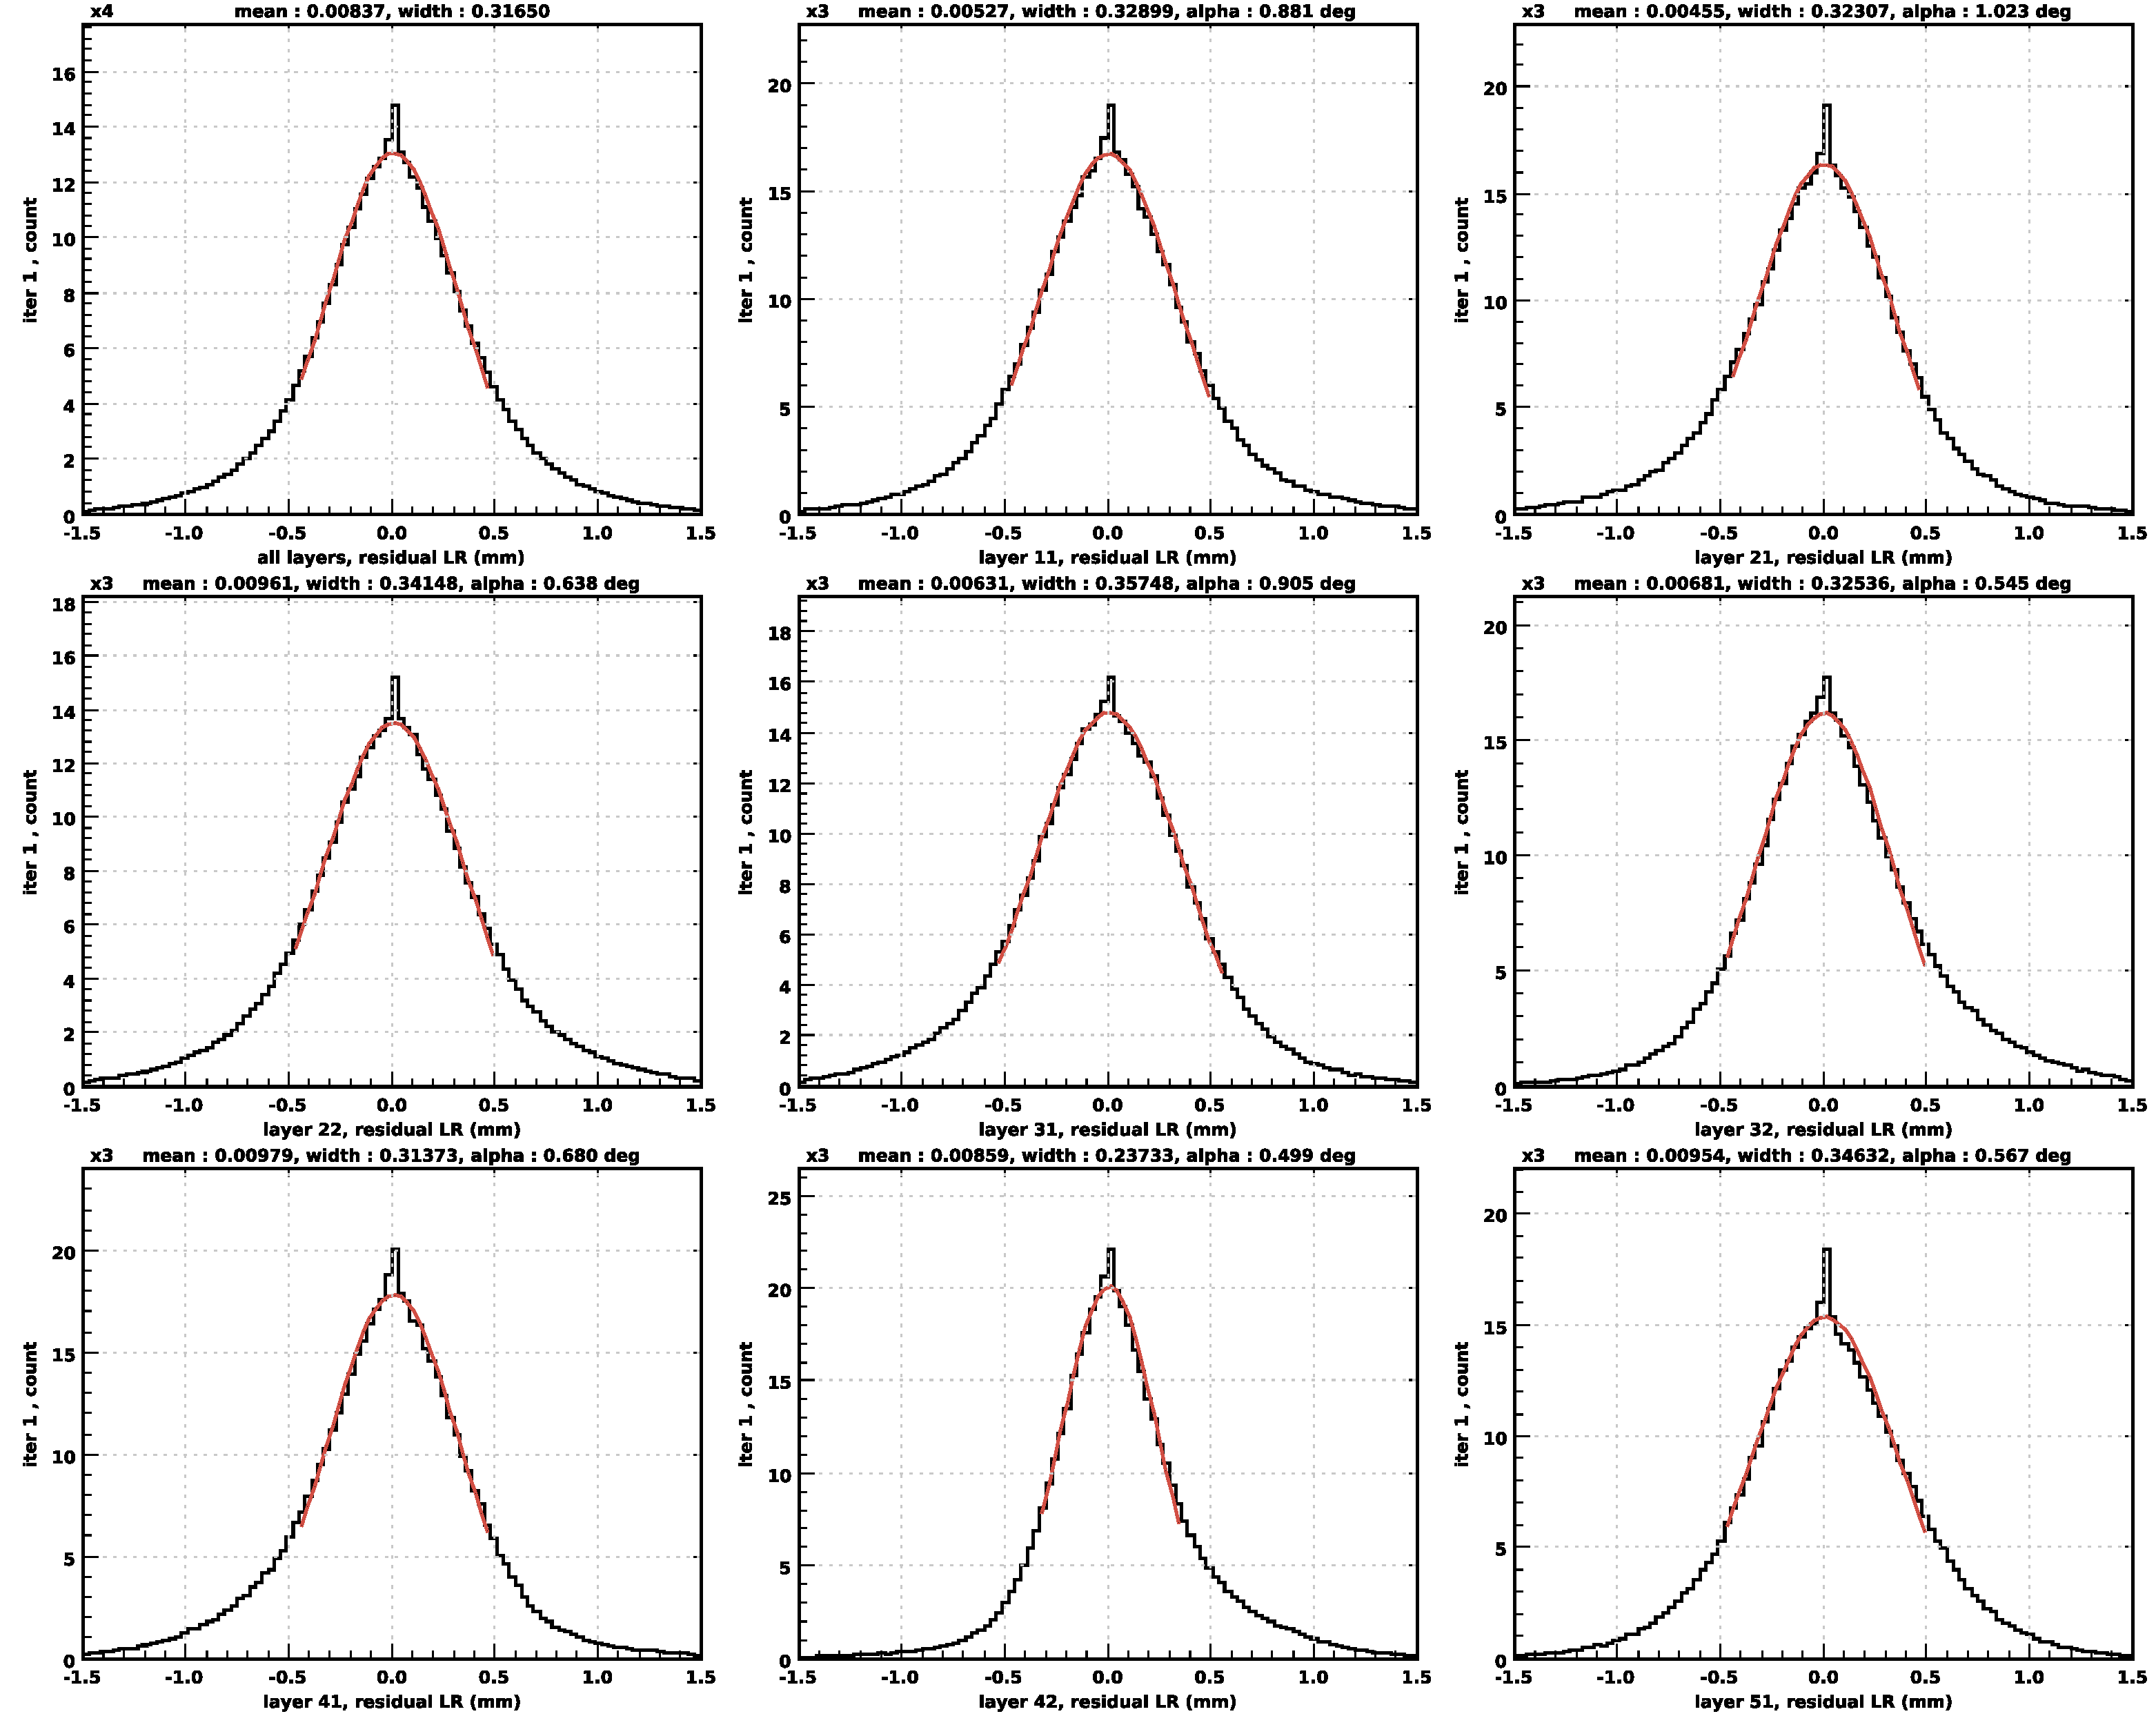
\includegraphics[width=\linewidth]{figures/residual_LR_iter_1_cb_v9.pdf}
    \end{minipage}
    
\end{frame}

\begin{frame}{Updates - layer alignment}
    \begin{itemize}
        \item For now, the rotation is the same for the two end points of the wires
        \item However, we have a correlation between the residual LR and the vz
        \item This let think that we should rotate the two end points independently
        %\item At the end the minimize the 
    \end{itemize}

    \vspace{0.05cm}
    \centering
    \begin{minipage}{0.7\textwidth}
        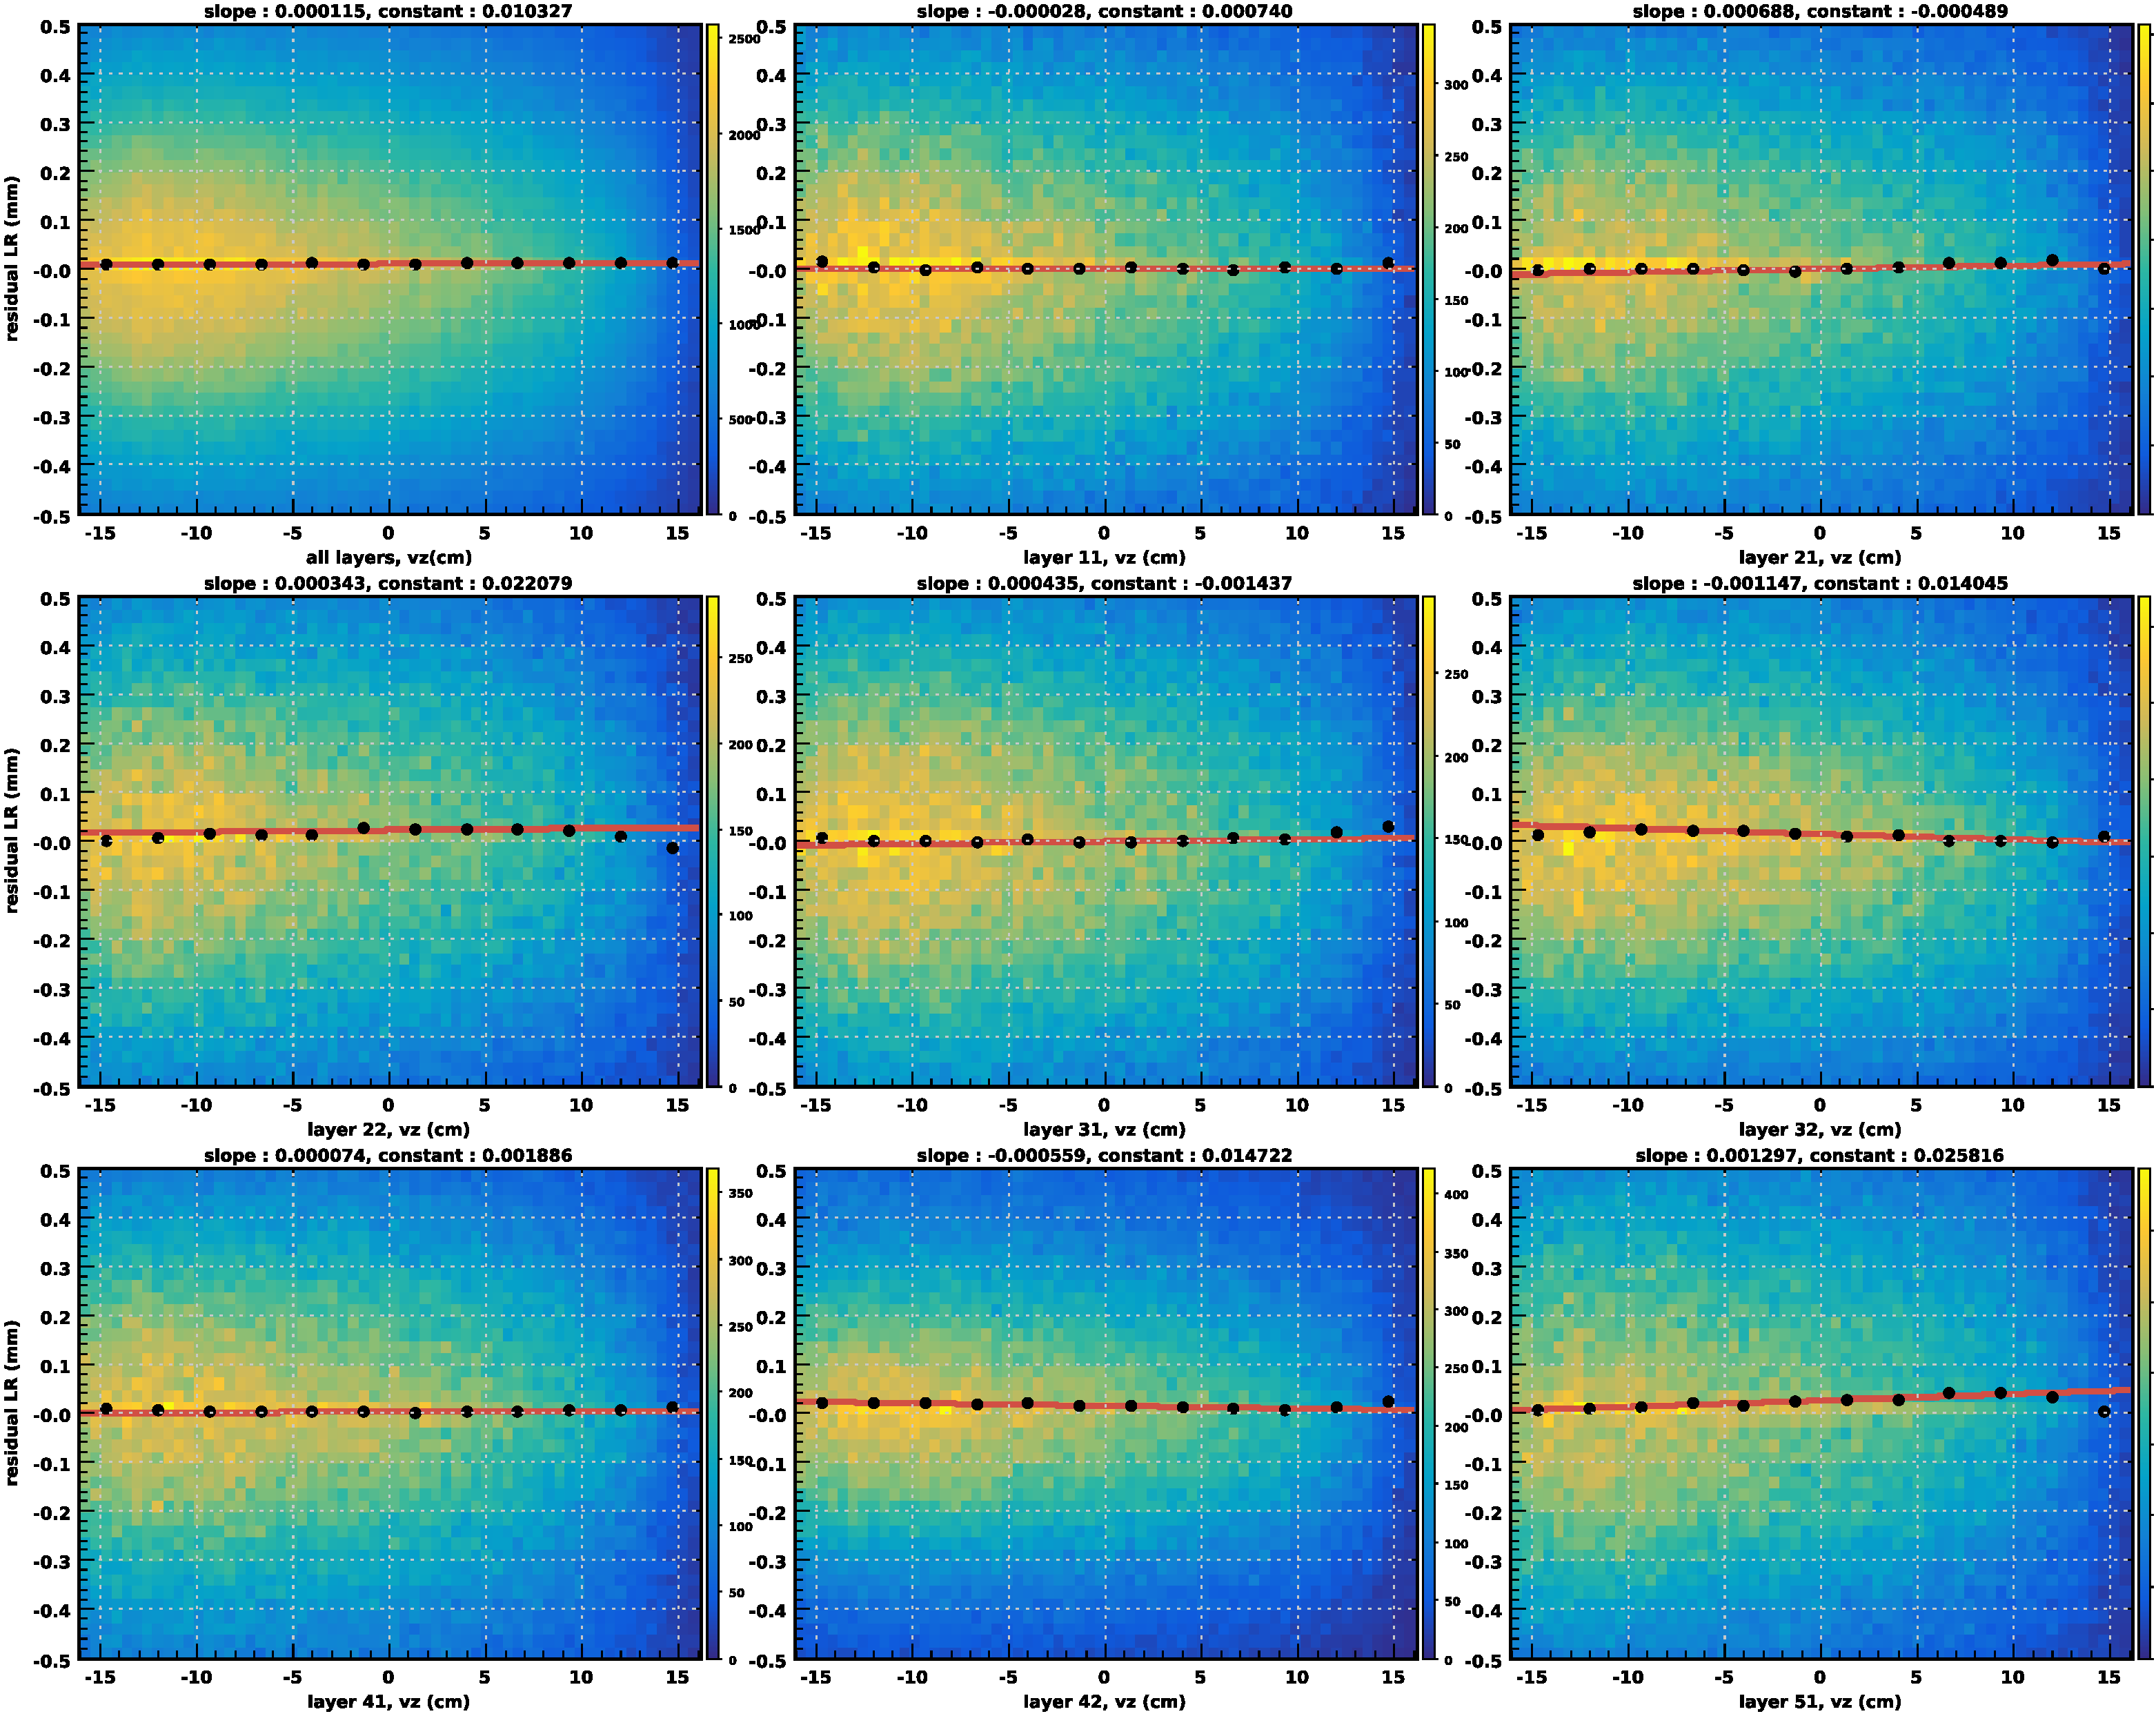
\includegraphics[width=\linewidth]{figures/corr_vz_residual_LR_iter_1_cb_v9.pdf}
    \end{minipage}
    
\end{frame}

\begin{frame}{Updates - vz alignment}
    \begin{itemize}
        \item We still need to determine the exact position of the AHDC with respect to CLAS
        \item Doing the alignment without KF fit, I noticed that the dispersion between the correction angles is more or less big depending on the AHDC position
        \item The values at vz = -70 mm are the most consistent here
    \end{itemize}

    \begin{center}
        \begin{tabular}{c|c|c|c}
            AHDC position & -54 mm $^($\footnote{hand made}$^)$ & -30 mm & -70 mm\\
            \hline
            layer 11 & 0     & -1.49 & +0.756 \\
            layer 21 & +2.55 & +3.82 & +1.517 \\
            layer 22 & +2.11 & +3.24 & +0.984 \\
            layer 31 & 0     & -1.54 & +0.807 \\
            layer 32 & -0.32 & -1.96 & +0.382 \\
            layer 41 & +3.0  & +3.73 & +1.305 \\
            layer 42 & +2.13 & +3.3  & +0.975 \\
            layer 51 & -0.21 & -1.61 & +0.679 \\
        \end{tabular}
    \end{center}

    % \vspace{0.2cm}
    % \centering
    % \begin{minipage}{0.8\textwidth}
    %     \includegraphics[width=\linewidth]{figures/build/position_scan.pdf}
    % \end{minipage}
    
    
\end{frame}

\begin{frame}{Updates - AHDC position scan}
    \begin{itemize}
        \item I did AHDC position scan
        \item Given this study, the optimal position is -75 mm. That's what I use for the alignment
        %\item At the end the minimize the 
    \end{itemize}

    \vspace{0.2cm}
    \centering
    \begin{minipage}{0.8\textwidth}
        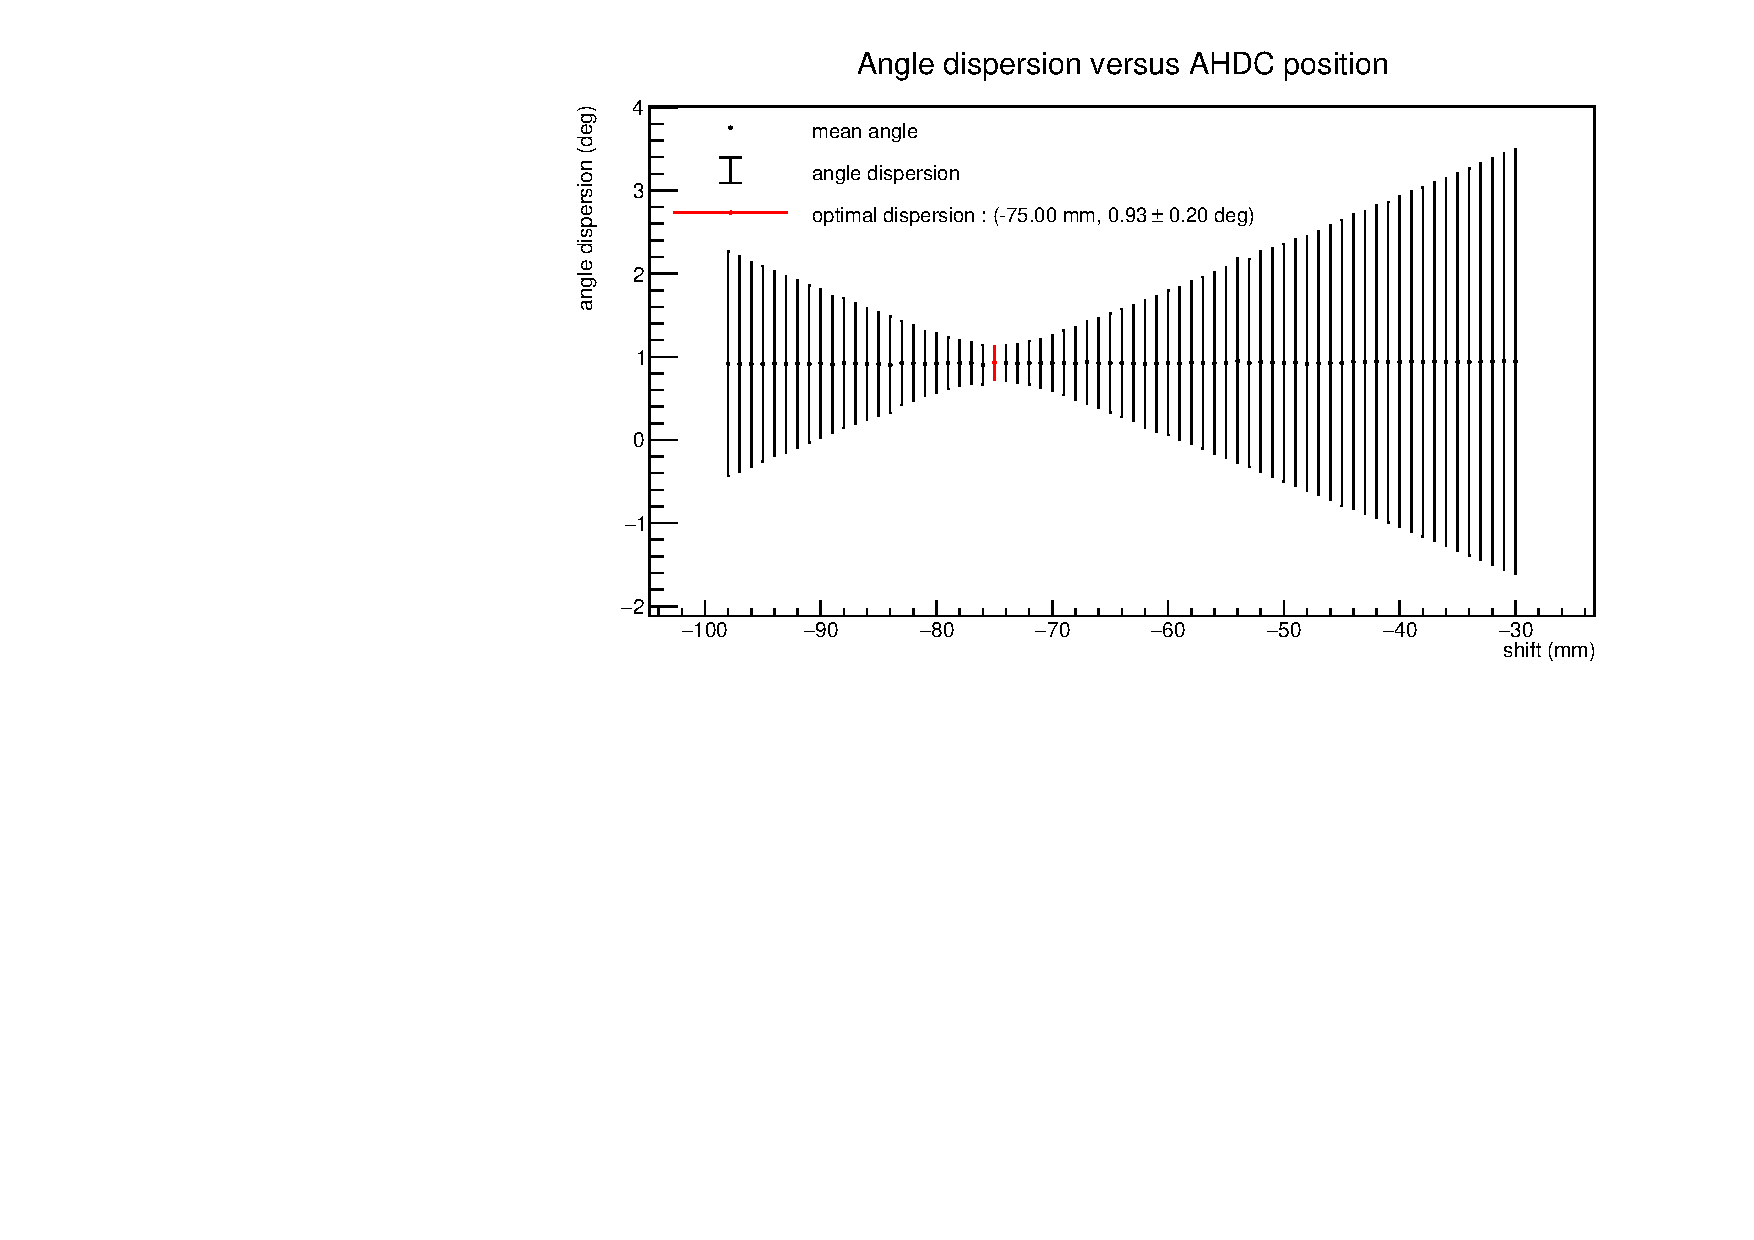
\includegraphics[width=\linewidth]{figures/ahdc_position_scan.pdf}
    \end{minipage}
    
\end{frame}

\begin{frame}{Next steps}
    \begin{itemize}
        \item I will continue my work on the alignment
            \begin{itemize}
                \item Rotate independently the two end points of the wires in a given layer
                \item Push the study further by doing a wire by wire alignment
            \end{itemize}
        \item Pending task
            \begin{itemize}
                \item Push my work on the ATOF hits for the Kalman Filter in coatjava
                \item Finish the work on the Kalman Filter (material verification, target gas density, PID, magnetic field, optimization)
            \end{itemize}
    \end{itemize}
    
\end{frame}



\begin{frame}{Backup slides}
    \begin{itemize}
        \item Procedure:
            \begin{enumerate}
                \item We looked at elastic events : electron + track (here: collection of hits only)
                \item We computed the theoretical momentum vector of the track $\vec{p}$
                \item We made the propagation without doing any fit (i.e no KF correction)
                \item We looked at {\color{blue} residual\_LR} (left-right) $\longrightarrow$ sensitive to the alignment
            \end{enumerate}
    \end{itemize}
    

    \vspace{0.2cm}
    \centering
    \begin{minipage}{0.42\textwidth}
        \includegraphics[width=\linewidth]{figures/build/illustration_residual_type.pdf}
    \end{minipage}

\end{frame}



% \begin{frame}{ATOF hit work completed 2/2}
%     \begin{itemize}
%         \item Status of the theta reconstruction
%         \item We have two peaks in the last version of the theta reconstruction
%             \begin{itemize}
%                 \item The first peak are tracks without ATOF matches
%                 \item The second peak around 86$^\circ$ are tracks with ATOF matches (45 \%)
%             \end{itemize}
%         \item The final 45 \% matches (over the nb. tracks) is low; it is essentially due the current misalignment between the AHDC and ATOF
%     \end{itemize}

%     \vspace{0.5cm}

%     \centering
%     \begin{minipage}{0.32\textwidth}
%         
\includegraphics[width=\linewidth]{figures/data_theta_new_geometry.pdf}
%     \end{minipage}
%     \begin{minipage}{0.32\textwidth}
%         
\includegraphics[width=\linewidth]{figures/data_theta_ai_matching.pdf}
%     \end{minipage}
%     \begin{minipage}{0.32\textwidth}
%         
\includegraphics[width=\linewidth]{figures/data_theta_proj_based_matching.pdf}
%     \end{minipage}







\end{document}


